\documentclass{winslabreport}
\reporttitle{An Implementation of BlindBox: Deep Packet Inspection
over Encrypted Traffic}
\coursename{CENG781 Network Security}
\courseterm{2018-2019 Spring}
\reportpurpose{Term Project Report}
\authorname{Cansin Yildiz, Fatma Demirtas, Seyma Bodur}
\studentnumber{1449271, 1927961, 1854512}
\useremail{cansin.yildiz@metu.edu.tr, fatma.demirtas@metu.edu.tr, bodur.seyma@metu.edu.tr}
\program{Computer Engineering}

\begin{document}
\restoregeometry
\maketitle
\tableofcontents
\listoffigures

\body

\section{Introduction}

Deep Packet Inspection (DPI), which is the computer network filtering technique, controls the content of the traffic and traffic flow \cite{Deep}. DPI is used in several areas such that protection to security threats, lawful interception, parental filtering. There are middleboxes to provide the functionality of DPI. In other words, Middleboxes should ensure security. However, there is a problem with some middleboxes: while providing security, they do not put emphasis on privacy. BlindBox, which is a middlebox presented in this report, provide both functionality of the DPI and privacy of the packets. If the BlindBox is used as middlebox, there is no need to decrypt the payload. Inspecting packets is made over encrypted payload. 

BlindBox ensures the following properties:

\begin{itemize}
	\item As all middleboxes do, BlindBox seek for suspicious content for security. 
	\item Sender and receiver do not have knowledge of the rule.
	\item BlindBox should have at least one trusted endpoint as in intrusion detection (IDS). 
	\item There is no permission for BlindBox to read the traffic unless there is no found suspicious content.
\end{itemize}

The last property is special for BlindBox, other middleboxes does not provide it.

Below figure shows how BlindBox works:

\begin{figure}[H]
	\centering
	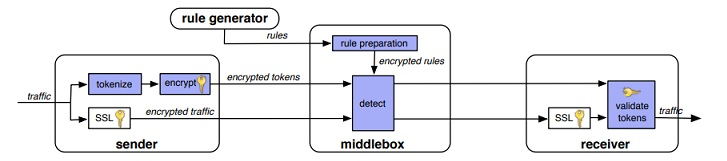
\includegraphics[width=150mm,height=35mm]{blindbox.jpg}
	\caption{BlindBox Architecture}
	\label{fig:bli1}
\end{figure}

There are three different keys to use in this scheme. First one is $k_{SSL}$ which is used in SSL protocol. The second one is k which is used for detection. The last one is $k_r$ and which is used for randomness. These three keys are generated/derived by $k_0$ which is the key sender and receiver agree by SSL Handshake. In that way, sender and receiver are connected.

As it is seen in the figure, there is a connection between the rule generator and the middlebox. Rule generator encrypts keywords/rules with the key k. And middlebox gets these rules to detect suspicious content without the knowledge of the key k. While this happening, endpoints should not have the knowledge of the rules, too.

After these connections, traffic should be encrypted with SSL by the sender as we can see in the Figure. Then, the sender starts to divide the traffic into substring to tokenize. These tokens are sent after encrypted with DPIEnc. DPIEnc works as

\begin{center}
	$salt ,  AES_{AES_k (t)}(salt)  mod RS$
\end{center}

where salt is random number, t is token, k is key and  RS which reduced the size of ciphertext is $2^{40}$

When the traffic comes to the middlebox, BlindBox Detect algorithm seek for a match between encrypted tokens and encrypted rules. If any suspicious content found in the traffic, it could be stopped or dropped as what is required. Otherwise, the traffic is sent to the receiver.

When the traffic comes to the receiver, it is decrypted and receiver authenticates the traffic using SSL. Also, the receiver controls whether encryption of the tokens is done correctly or not. 

\section{Related Work}

There are many related works on middleboxes. Some of them are accepted insecure. As explained in \cite{SSL} , man in the middle attack is built using counterfeit certificates on SSL by some systems. In that way, security of the SSL could be broken, and middlebox can decrypt the traffic for detection scan. That is, E2E security of SSL is destroyed which is insecure. In addition, there is a system called Meddle \cite{Traffic}. Its goal is to increase transparency in mobile networks. This is done by endpoints and the third-party are authorized to control the traffic, which is not required in BlindBox. The systems APLOMB \cite{Network} and Beyond the Radio \cite{48} are similar to Meddle.

Some middleboxes use encrypted payload for detection. But, they have some properties that are not required for BlindBox. For example,  fully homomorphic encryption\cite{24} and general functional encryption \cite{23} can be used in order to encrypt the payload. Their computation speed is so slow when they are compared with an encryption scheme used in BlindBox.

Also, searchable encryption schemes can be used in order to encrypt the rules. However, such schemes encrypt the rules in such a way that it does not meet the security which BlindBox require. In addition, symmetric key searchable scheme \cite{46} and public key encryption with searching  \cite{19} can also be used for packet processing. However, they have some weakness: symmetric key searchable scheme is slower than the scheme which BlindBox uses, and the public key searchable scheme is also not proper for performance because it should create cryptographic pairs for each token.

All these means, security and speed desires cannot be obtained by all these encryption schemes. Therefore, BlindBox uses different encryption scheme which is called DPIEnc. DPIEnc takes the speed of deterministic searchable encryption scheme and it takes the security of the randomized encryption scheme.   

\appendix

\section{P4 Tutorial Result}

As a P4 tutorial, we selected the \emph{basic} exercise. The objective of the exercise is to implement basic forwarding for IPv4. As most of the other resources lack a detailed explanation of the P4 language, we ended up simply copying the exercise's solution over and reading it, in order to understand the language more.

After a short evaluation, we got more comfortable with the language and decided to augment the tutorial. The final result of what we have worked on can be found at our GitHub repository at \cite{groupf}. 

We realized there are multiple moving parts for a P4 project. The \emph{topology.json} and \emph{*runtime.json} files together define the network setup for Mininet \cite{Lantz:2010:NLR:1868447.1868466}, while the main \emph{*.p4} file contains the middlebox implementation. In order to simplify the network setup, we stripped down the \emph{*.json} files to have a directed minimal 2-client-1-switch setup.

Later we incorporated a \emph{TCP} header extraction step to the parser. In order to do so, we simply introduced a new header type \emph{tcp\_t}, and added a new \emph{tcp} header section to our \emph{headers} struct with the type. Parsing this new header was as simple as introducing a new \emph{parse\_tcp} state to our parser and emitting it back in deparser, as shown in \ref{lst:parser}.

\begin{lstlisting}[caption={P4 parser snippet},label={lst:parser},language=C]
const bit<8> TYPE_TCP = 0x06;

// Parser

state parse_ipv4 {
    packet.extract(hdr.ipv4);
    transition select(hdr.ipv4.protocol) {
        TYPE_TCP: parse_tcp;
        default: accept;
    }
}

state parse_tcp {
    packet.extract(hdr.tcp);
    transition accept;
}

// Deparser

packet.emit(hdr.ipv4);
packet.emit(hdr.tcp);
\end{lstlisting}

We also spent some time working on the given client code by the exercise. Since the backbone of the BlindBox implementation relies heavily on \emph{AES}, we decided to augment the given sender/receiver pair to encrypt/decrypt the message sent over. In order to do so, we first converted the Python implementation to be package-based in order to utilize a shared \emph{aes.py} code by both the sender and the receiver. 

Having such a single implementation was needed in order to have a shared \emph{key} and \emph{initial\_value} between the receiver and the sender, and also to centralize the effort needed in order to pad given messages' length to be a multiple of 16 (which is a requirement for AES). As shown in \ref{lst:aes}, we utilized \emph{pycrypto} library for AES implementation.

\begin{lstlisting}[caption={AES encryption/decryption},label={lst:aes},language=Python]
import math

from Crypto.Cipher import AES

KEY = 'DEB536FA9890D43BEED9654AF0DBFC6A'
INITIAL_VALUE = '6C0AF5F86C504961204B1A42D8B99530'

aes = AES.new(KEY, AES.MODE_CBC, INITIAL_VALUE)

def encrypt(text):
    padding_threshold = int(math.ceil(len(text) / 16.0) * 16)
    return aes.encrypt(text.ljust(padding_threshold))

def decrypt(cipher_text):
    return aes.decrypt(cipher_text).rstrip()
\end{lstlisting}

We believe this exercise was a good starting point for us to implement BlindBox. We also spent some time trying to figure out how we can read the payload of a given TCP packet, but after spending some time, we realized the P4 language is actually not intended to be used with arbitrarily sized packet payloads. Instead, it is all about packet \emph{headers}. 

So, in order to implement the tokenizer protocol, we are now considering creating a custom protocol on top of TCP that would have a fixed-16-size \emph{token} header that our P4 middlebox implementation can parse and match against a given list of possible offending \emph{rules}.

\bibliographystyle{plain}
\bibliography{references}
\end{document}
